\section{Testing della Versione 5}

%%%%%%%%%%%%%%%%%%%%%%%%%%%%%%%%%%%%%%%%%%
%          TEST CLASSE CATEGORIA         %
%%%%%%%%%%%%%%%%%%%%%%%%%%%%%%%%%%%%%%%%%%

\begin{frame}{Test Classe Categoria}
    \framesubtitle{Test di classe}
    Per il test di classe della versione 5 abbiamo selezionato la classe Categoria in quanto permetteva di effettuare in modo efficiente test su numerosi metodi.\\\bigskip
    Sarebbe diversamente stato complesso testare classi che richiedessero l'input da parte dell'utente.
\end{frame}

\begin{frame}{Test Classe Categoria}
    \framesubtitle{Test di classe}
    
    \begin{figure}
        \centering
        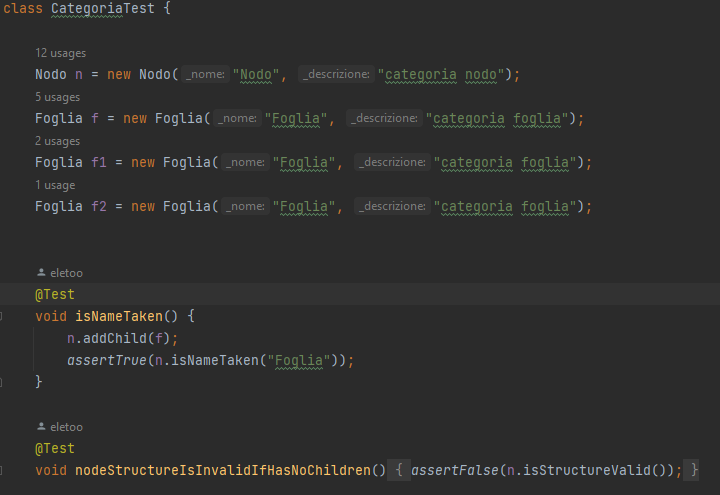
\includegraphics[width=.7\textwidth]{initial testing/initialtesting-categoria1.png}
    \end{figure}    

    \note{
        Disclaimer: il codice della versione 5 era particolarmente disorganizzato e non rispettava alcun pattern. \\
        Con la versione finale post-refactoring è chiaramente più facile testare in modo più ordinato non solo questa classe ma anche tutte le altre.\\\bigskip
        I test effettuati hanno nomi esplicativi relativamente al fine del test stesso.
    }
\end{frame}
        
\begin{frame}{Test Classe Categoria}
    \begin{figure}
        \centering
        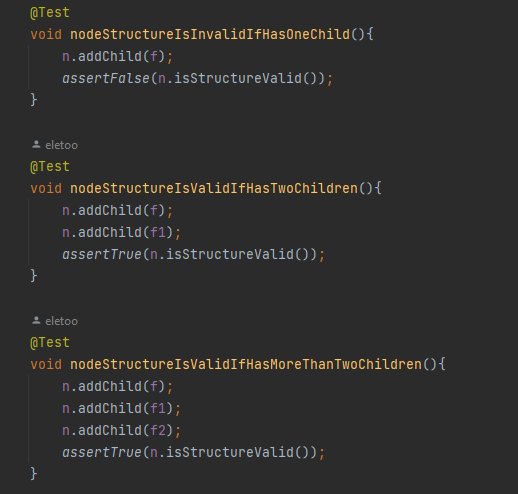
\includegraphics[width=.5\textwidth]{initial testing/initialtesting-categoria2.png}
        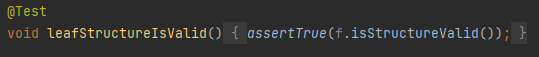
\includegraphics[width=.7\textwidth]{initial testing/initialtesting-categoria3.png}
    \end{figure}    
\end{frame}


%%%%%%%%%%%%%%%%%%%%%%%%%%%%%%%%%%%%%%%%%%
%          TEST CLASSE ORARIO            %
%%%%%%%%%%%%%%%%%%%%%%%%%%%%%%%%%%%%%%%%%%
\begin{frame}{Test Classe Orario}
    \framesubtitle{Test di requisiti e funzionalità}
    Per il test delle funzionalità abbiamo selezionato la funzionalità:\\
    ``Gli orari per effettuare lo scambio possono essere solo allo scoccare dell'ora o alla mezza (ogni trenta minuti)''\\\bigskip
    Abbiamo applicato volutamente un testing ``superficiale'' sulla versione 5 in modo da poter mostrare l'evoluzione tra l'inizio e la fine del progetto della tecnica utilizzata per individuare i casi di test
    
\end{frame} 

\begin{frame}{Test Classe Orario}
    \framesubtitle{Test di requisiti e funzionalità}
    
    \begin{figure}
        \centering
        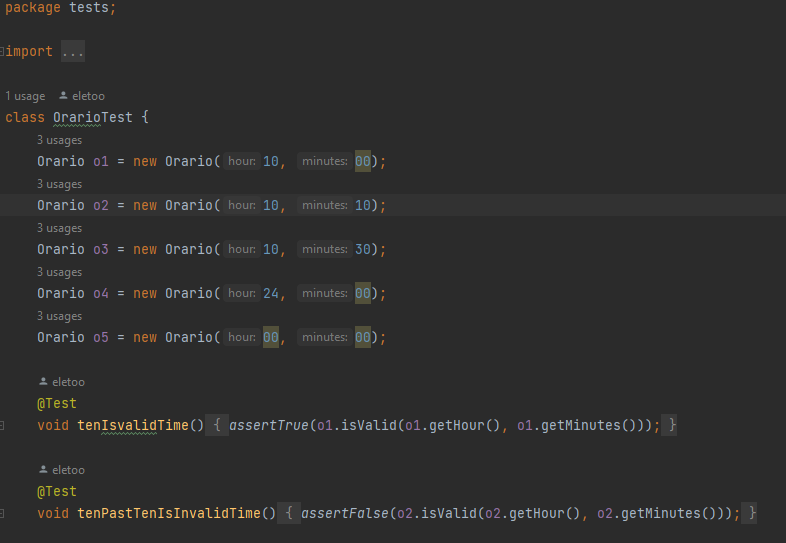
\includegraphics[width=.7\textwidth]{initial testing/initialtestingorario1.png}
    \end{figure}    

    \note{
        Inizialmente i casi di test individuati erano in numero ridotto e poco approfonditi, mentre il testing della versione finale post-refactoring, come si vedrà nella sezione finale della presentazione, è stato effettuato in maniera più precisa e tenendo conto delle linee guida per l'individuazione dei casi di test black box. 
    }

\end{frame}

\begin{frame}{Test Classe Orario}
    \begin{figure}
        \centering
        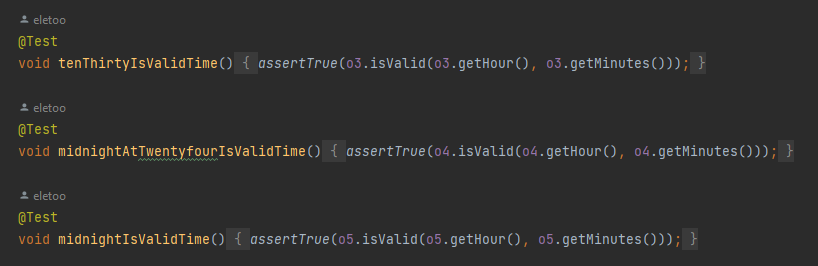
\includegraphics[width=.8\textwidth]{initial testing/initialtestingorario2.png}
    \end{figure}
\end{frame}